\subsection{Kasseapparat}

Kasseapparatet blev opbygget med tre lags strukturen: Presentation-, Business logic- og Data Access Layer. Disse lag vil blive beskrevet i nedenstående afsnit.

\subsubsection{Designovervejelser}
Designet af Kasseapparatet blev startet ved at der blev tegnet en skitse for hvordan selve brugergrænsefladen skulle ende med at se ud.
Det var vigtigt at der en klar opdeling af de forskellige lag. Dette betød at der mellem præsentations- og business logic laget blev benyttet MVVM. MVVM er et pattern, der sikrer at kommunikationen mellem grænsefladen og underliggende Viewmodels er håndteret ordentligt. \\
Det første der blev implementeret til Kasseapparatet var selve grænsefladen. Grænsefladen blev opstillet med knapper uden nogen funktionalitet. Herefter begyndte funktionaliteten at blive implementeret. Funktionaliteten startede ud som en klasse der kunne indholde de tilgængelige produkter, samt en fake af database connectionen, som kunne fylde denne liste med dummie produkter, hvilket lettede videre udvikling da der allerede kunne testes med produkter. Herefter kunne arbejdet deles i repræsentation af produkter i gui'en, og håndtering af indkøbskurven samt egentlige forbindelse til CentralServer

\subsubsection{Presentation Layer}

Det første der blev opsat til kasseapparatet var grænsefladen. Dette kan virke lidt bagvendt, men det var fra starten et fokus at skabe et anderledes kasseapparat der var nemt at benytte sig af. Med dette menes der et program med en klar vej fra start til slut. Der måtte gerne være flere måder at gennemføre salg på, men brugeren måtte ikke være tvunget til at benytte sig af allesammen.
Først blev der opsat en skitse, se figur, hvor kasseapparatet var delt op i 3 segmenter. Her var idéen at produkterne skulle være i segmentet på venstre side, indkøbskurven i midten, og knapperne til brug i betalingen på højre side. Derved ville et salg gå fra højre i mod venstre i det at man først ville tilføje et produkter i venstre side. Disse ville komme frem i midten, og til sidst ville betalingen blive gennemført i højre side af kasseapparatet. 

\begin{figure}[H]
	\centering
	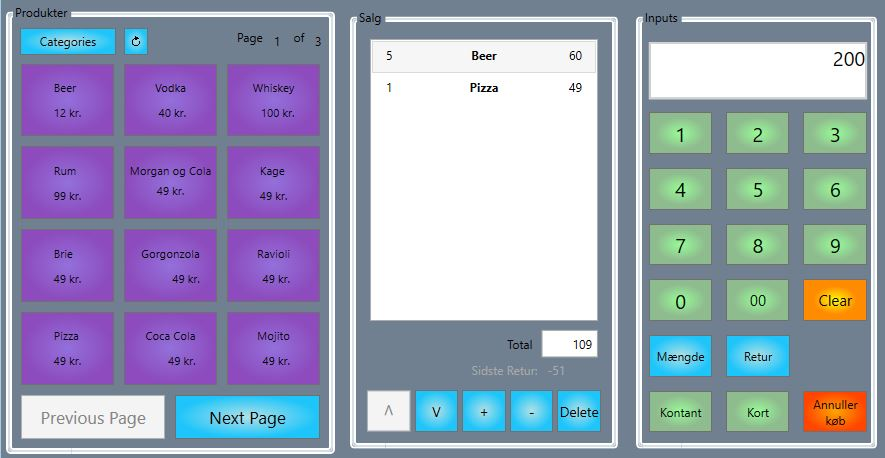
\includegraphics[width=0.9\linewidth]{Projektbeskrivelse/DesignOgImplementering/pics/GUI}
	\caption{Endelig Implementering}
	\label{fig:sub2}
\end{figure}

Som man kan se på figur \ref*{fig:sub2} så blev grænsefladen udviklet relativt tæt på skitsen, dog med nogle flere knapper i betalingssegmentet. For at sikre at der var mange måder at tilføje produkter på, blev det lavet sådan at man kunne tilføje et produkt ved at klikke gentagne gange på hver produkt. Samtidig kan man trykke et et tilføjet produkt, skrive et antal i betalingsdelen og trykke på mængde. Så vil den angivne mængde af produkter blive tilføjet. \\

\textbf{Knapper og sideskift} \\
Noget der er lagt meget tid i, er knappeskift. Dette blev implementeret ved at oprette et kontrolobjekt til knapper\footnote{ProductButtonControl}. Dette objekt indeholder en liste der inderholder liste af 12 knapper. Derved kan der nemt skiftes side af knapper bare ved at ændre den liste der vises på kasseapparatet.
\subsection{Busines Logic Layer}
\subsection{Data Access Layer}

